\documentclass[10pt]{article}
\usepackage[utf8]{inputenc}
\usepackage[T1]{fontenc}
\usepackage{amsmath}
\usepackage{amsfonts}
\usepackage{amssymb}
\usepackage[version=4]{mhchem}
\usepackage{stmaryrd}
\usepackage{graphicx}
\usepackage[export]{adjustbox}
\graphicspath{ {./images/} }
\usepackage{bbold}

\title{Maximum Likelihood }

\author{}
\date{}


\begin{document}
\maketitle
Machine Learning Course - CS-433

Oct 4, 2023

Martin Jaggi

Last updated on: October 3, 2023

credits to Mohammad Emtiyaz Khan \& Rüdiger Urbanke

$$
\text { EPFL }
$$

\section*{Motivation}
In the previous lecture $3 \mathrm{a}$ we arrived at the least-squares problem in the following way: we postulated a particular cost function (square loss) and then, given data, found that model that minimizes this cost function. In the current lecture we will take an alternative route. The final answer will be the same, but our starting point will be probabilistic. In this way we find a second interpretation of the least-squares problem.
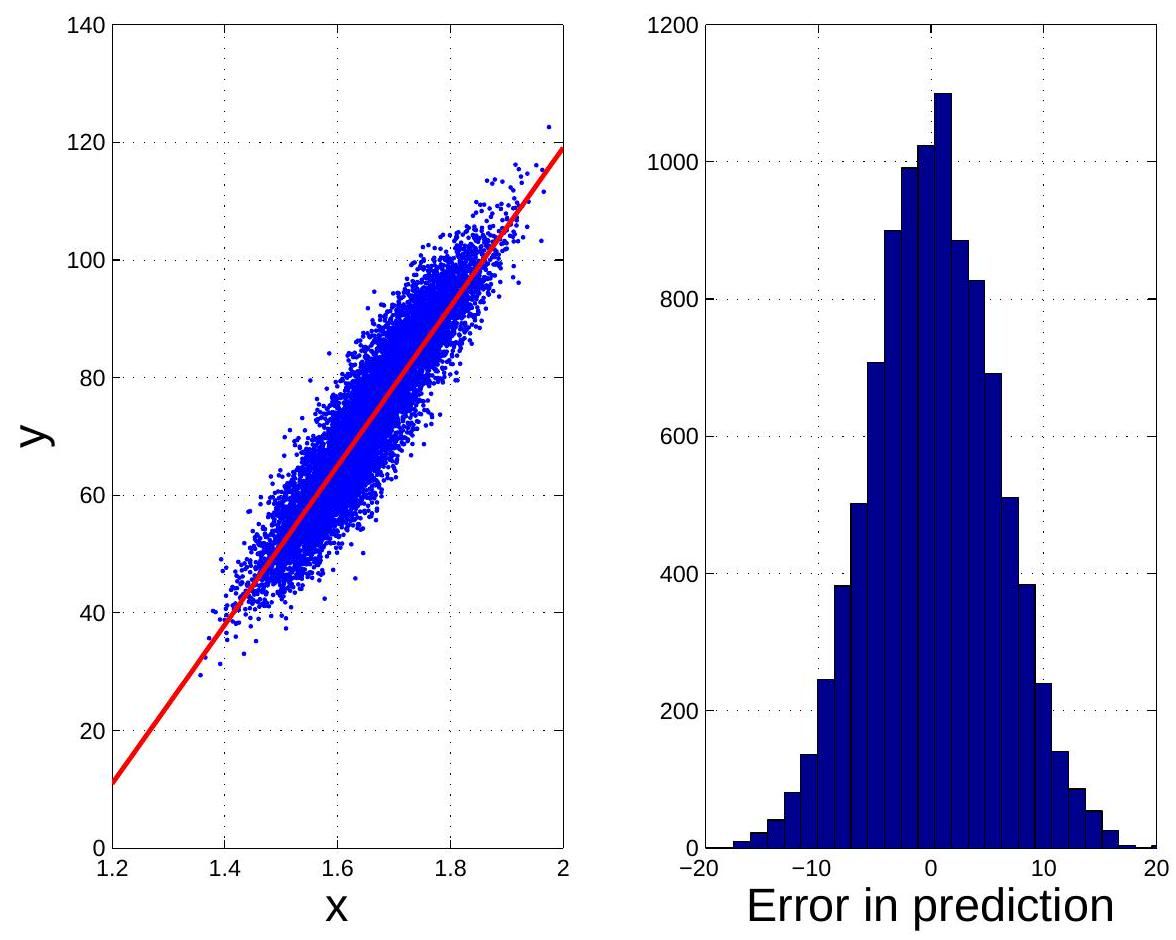
\includegraphics[max width=\textwidth, center]{2023_12_30_b8ee6e6de203e1077c28g-2}

\section*{Gaussian distribution and independence}
Recall the definition of a Gaussian

random variable in $\mathbb{R}$ with mean $\mu$ and variance $\sigma^{2}$. It has a density of

$p\left(y \mid \mu, \sigma^{2}\right)=\mathcal{N}\left(y \mid \mu, \sigma^{2}\right)=\frac{1}{\sqrt{2 \pi \sigma^{2}}} \exp \left[-\frac{(y-\mu)^{2}}{2 \sigma^{2}}\right]$.

In a similar manner, the density of a

Gaussian random vector with mean

$\boldsymbol{\mu}$ and covariance $\boldsymbol{\Sigma}$ (which must be

a positive semi-definite matrix) is

$\mathcal{N}(\mathbf{y} \mid \boldsymbol{\mu}, \boldsymbol{\Sigma})=\frac{1}{\sqrt{(2 \pi)^{D} \operatorname{det}(\boldsymbol{\Sigma})}} \exp \left[-\frac{1}{2}(\mathbf{y}-\boldsymbol{\mu})^{\top} \boldsymbol{\Sigma}^{-1}(\mathbf{y}-\boldsymbol{\mu})\right]$.

Also recall that two random vari-

ables $X$ and $Y$ are called indepen-

dent when $p(x, y)=p(x) p(y)$.

\section*{A probabilistic model for least-squares}
We assume that our data is generated by the model,

$$
y_{n}=\mathbf{x}_{n}^{\top} \mathbf{w}+\epsilon_{n}
$$

where the $\epsilon_{n}$ (the noise) is a zeromean Gaussian random variable with variance $\sigma^{2}$ and the noise that is added to the various samples is independent of each other, and independent of the input. Note that the model $\mathbf{w}$ is unknown.

Therefore, given $N$ samples, the likelihood of the data vector $\mathbf{y}=$ $\left(y_{1}, \cdots, y_{N}\right)$ given the input $\mathbf{X}$ (each row is one input) and the model $\mathbf{w}$ is equal to

$p(\mathbf{y} \mid \mathbf{X}, \mathbf{w})=\prod_{n=1}^{N} p\left(y_{n} \mid \mathbf{x}_{n}, \mathbf{w}\right)=\prod_{n=1}^{N} \mathcal{N}\left(y_{n} \mid \mathbf{x}_{n}^{\top} \mathbf{w}, \sigma^{2}\right)$.

The probabilistic view point is that we should maximize this likelihood over the choice of model w. I.e., the "best" model is the one that maximizes this likelihood.

\section*{Defining cost with log-likelihood}
Instead of maximizing the likelihood, we can take the logarithm of the likelihood and maximize it instead. Expression is called the loglikelihood (LL).

$\mathcal{L}_{\mathrm{LL}}(\mathbf{w}):=\log p(\mathbf{y} \mid \mathbf{X}, \mathbf{w})=-\frac{1}{2 \sigma^{2}} \sum_{n=1}^{N}\left(y_{n}-\mathbf{x}_{n}^{\top} \mathbf{w}\right)^{2}+$ cnst.

Compare the LL to the MSE (mean squared error)

$$
\begin{aligned}
\mathcal{L}_{\mathrm{LL}}(\mathbf{w}) & =-\frac{1}{2 \sigma^{2}} \sum_{n=1}^{N}\left(y_{n}-\mathbf{x}_{n}^{\top} \mathbf{w}\right)^{2}+\mathrm{cnst} \\
\mathcal{L}_{\mathrm{MSE}}(\mathbf{w}) & =\frac{1}{2 N} \sum_{n=1}^{N}\left(y_{n}-\mathbf{x}_{n}^{\top} \mathbf{w}\right)^{2}
\end{aligned}
$$

\section*{Maximum-likelihood estimator (MLE)}
It is clear that maximizing the LL is equivalent to minimizing the MSE:

$\arg \min _{\mathbf{w}} \mathcal{L}_{\mathrm{MSE}}(\mathbf{w})=\arg \max _{\mathbf{w}} \mathcal{L}_{\mathrm{LL}}(\mathbf{w})$.

This gives us another way to design cost functions.

MLE can also be interpreted as finding the model under which the observed data is most likely to have been generated from (probabilistically). This interpretation has some advantages that we discuss now.

\section*{Properties of MLE}
MLE is a sample approximation to the expected log-likelihood:

$$
\mathcal{L}_{\mathrm{LL}}(\mathbf{w}) \approx \mathbb{E}_{p(y, \mathbf{x})}[\log p(y \mid \mathbf{x}, \mathbf{w})]
$$

MLE is consistent, i.e., it will give us the correct model assuming that we have a sufficient amount of data. (can be proven under some weak conditions)

$\mathbf{w}_{\text {MLE }} \longrightarrow^{p} \mathbf{w}_{\text {true }} \quad$ in probability

The MLE is asymptotically normal, i.e.,

$\left(\mathbf{w}_{\text {MLE }}-\mathbf{w}_{\text {true }}\right) \longrightarrow^{d} \frac{1}{\sqrt{N}} \mathcal{N}\left(\mathbf{w}_{\text {MLE }} \mid \mathbf{0}, \mathbf{F}^{-1}\left(\mathbf{w}_{\text {true }}\right)\right)$

where $\mathbf{F}(\mathbf{w})=-\mathbb{E}_{p(\mathbf{y})}\left[\frac{\partial^{2} \mathcal{L}}{\partial \mathbf{w} \partial \mathbf{w}^{\top}}\right]$ is the Fisher information.

MLE is efficient, i.e. it achieves the Cramer-Rao lower bound.

Covariance $\left(\mathbf{w}_{\text {MLE }}\right)=\mathbf{F}^{-1}\left(\mathbf{w}_{\text {true }}\right)$

\section*{Another example}
We can replace Gaussian distribu-

tion by a Laplace distribution.

$$
p\left(y_{n} \mid \mathbf{x}_{n}, \mathbf{w}\right)=\frac{1}{2 b} e^{-\frac{1}{b}\left|y_{n}-\mathbf{x}_{n}^{\top} \mathbf{w}\right|}
$$


\end{document}